% #######################################
% ########### FILL THESE IN #############
% #######################################
\def\mytitle{Distributive law proof using Arduino}
\def\mykeywords{}
\def\myauthor{P.Sravan kumar}
\def\contact{sravankumar912126@gmail.com}
\def\mymodule{Future Wireless Communications-(FWC22043)}
% #######################################
% #### YOU DON'T NEED TO TOUCH BELOW ####
% #######################################
\documentclass[10pt, a4paper]{article}
\usepackage[a4paper,outer=1.5cm,inner=1.5cm,top=1.75cm,bottom=1.5cm]{geometry}
\twocolumn
\usepackage{graphicx}
\graphicspath{{./images/}}
%colour our links, remove weird boxes
\usepackage[colorlinks,linkcolor={black},citecolor={blue!80!black},urlcolor={blue!80!black}]{hyperref}
%Stop indentation on new paragraphs
\usepackage[parfill]{parskip}
%% Arial-like font
\usepackage{lmodern}
\renewcommand*\familydefault{\sfdefault}
%Napier logo top right
\usepackage{watermark}
%Lorem Ipusm dolor please don't leave any in you final report ;)
\usepackage{lipsum}
\usepackage{xcolor}
\usepackage{listings}
%give us the Capital H that we all know and love
\usepackage{float}
%tone down the line spacing after section titles
\usepackage{titlesec}
%Cool maths printing
\usepackage{amsmath}
%PseudoCode
\usepackage{algorithm2e}

\titlespacing{\subsection}{0pt}{\parskip}{-3pt}
\titlespacing{\subsubsection}{0pt}{\parskip}{-\parskip}
\titlespacing{\paragraph}{0pt}{\parskip}{\parskip}
\newcommand{\figuremacro}[5]{
    \begin{figure}[#1]
        \centering
        \includegraphics[width=#5\columnwidth]{#2}
        \caption[#3]{\textbf{#3}#4}
        \label{fig:#2}
    \end{figure}
}

\lstset{
	frame=single, 
breaklines=true,
columns=fullflexible
}

\thiswatermark{\centering \put(0,-90.0){
\includegraphics[scale=0.05]{iith.jpg}} }
\title{\mytitle}
\author{\myauthor\hspace{1em}\\\contact\\IITH\hspace{0.5em}-\hspace{0.5em}\mymodule}
\date{}
\hypersetup{pdfauthor=\myauthor,pdftitle=\mytitle,pdfkeywords=\mykeywords}
\sloppy
% #######################################
% ########### START FROM HERE ###########
% #######################################
\begin{document}
	\maketitle
\tableofcontents

\section{Introduction}

There are different type of boolean algebra rules to simplify the boolean expression.One of the important law is distributive law.This can be stated as follows:
         A.(B+C)=A.B+A.C (OR distributive law).
         A+(B.C)=(A+B).(A+C) (AND distributive law).


\section{Method to solve}


To prove distributive law I used seven segment display and 7447 Ic to control it using binary.Take 3 variables a,b,c and take another 2 variables x,y for LHS (A.(B + C)) and RHS (A.B + A.C). 

If they are equal the seven segment display display's 1 else display's 0. By changing three boolean variables we can observe the distributive law satisfies or not for different inputs.Like these we can prove the distributive law.

code link :
 \begin{lstlisting}
    https://github.com/Sravan24365/iith-fwc/blob/main/assign1/codes/ass1.txt
\end{lstlisting}

\section{Components}



\begin{table}[htbp]
 \begin{center}
    \begin{tabular}{|l|c|c|c|c|c|c} \hline \textbf{Component}
  & \textbf{value} & \textbf{quantity} \\
 \hline
Resistor & 220 ohm & 1 \\ \hline
Arduino & UNO & 1 \\ \hline
sevensegment display &  & 1 \\ \hline
decoder & 7447 & 1  \\ \hline
Bread board &  & 1 \\ \hline
Jumper wires & M-M & 20\\ \hline
\end{tabular}   
\end{center}
\caption{\label{table:dummytable} }
\end{table}


\section{Distributive law proof with truth table}
.


\begin{table}[htbp]
 \begin{center}
    \begin{tabular}{|l|c|c|c|c|c|c|c|c} \hline \textbf{A}
  & \textbf{B} & \textbf{C} & \textbf{x(LHS)}& \textbf{y(RHS)} \\
 \hline
0&0&0&0&0 \\ \hline
0&0&1&0&0 \\ \hline
0&1&0&0&0\\ \hline
0&1&1&0&0  \\ \hline
1&0&0&0&0 \\ \hline
1&0&1&1&1\\ \hline
1&1&0&1&1\\ \hline
1&1&1&1&1\\ \hline
\end{tabular}   
\end{center}
\caption{\label{table:dummytable} }
\end{table}







\section{Connections}

Make connections to the Sevensegment display and 7447 IC based on table 3 and figure 1.


\begin{table}[htbp]
 \begin{center}
    \begin{tabular}{|l|c|c|c|c|c|c|c|c} \hline \textbf{7447}
  & \textbf{a'} & \textbf{b'} & \textbf{c'}& \textbf{d'}& \textbf{e'}& \textbf{f'}& \textbf{g'} \\
 \hline
Display&a&b&c&d&e&f&g \\ \hline

\end{tabular}   
\end{center}
\caption{\label{table:dummytable} }
\end{table}



\begin{center}

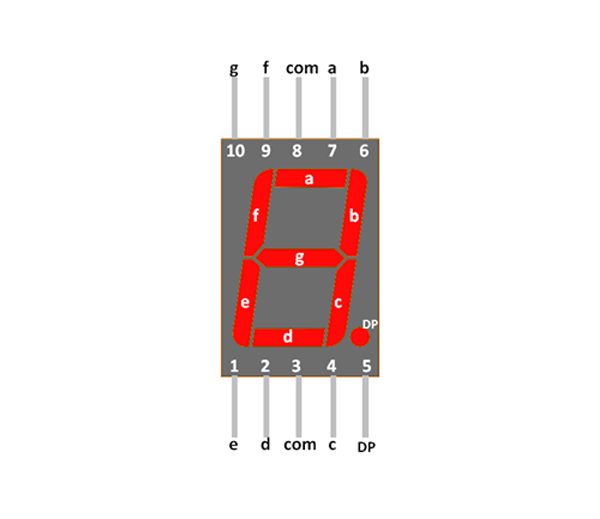
\includegraphics[scale=.20]{lcde.png}
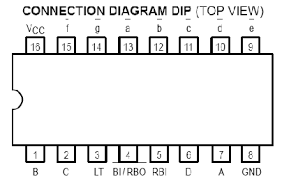
\includegraphics[scale=.20]{7447.png}


\end{center}
Figure 1:Sevensegment and 7447 IC.

Also make connections to arduino UNO ,7447 IC and inputs based on table 5

\begin{table}[htbp]
 \begin{center}
    \begin{tabular}{|l|c|c|c|c|c|c|c|c} \hline \textbf{Arduino UNO}
  & \textbf{2} & \textbf{3} & \textbf{4}& \textbf{5}& \textbf{6}& \textbf{7}& \textbf{8} \\
 \hline
7447&A&B&C&D&&& \\ \hline
input&&&&&k&l&m \\ \hline

\end{tabular}   
\end{center}
\caption{\label{table:dummytable} }
\end{table}
\section{Conclusion}
The output of sevenseg  is 1 for all possible inputs.So x=y i.e  A.(B+C)=A.B+A.C hence distributive law verfied.
\end{document}